\chapter{The LHC and ATLAS Experiment}
\quoteAuthor{You can observe a lot by watching.}{Yogi Berra}

\section{The Large Hadron Collider}
The \gls{LHC} \cite{lhc} is a hadron accelerator and collider 27 km in circumference located on the French-Swiss border. It collides beams of protons\footnote{The LHC also collides ions to study lead-lead (PbPb) as well as proton-lead interactions} at high rate and center-of-mass energy. In \RunTwo, which spanned from 2015 to 2018, the \gls{come} in the laboratory frame was 13 TeV (6.5 TeV per beam), and bunches of about $10^{11}$ protons collided every 25 ns.

Hydrogen atoms are the source of the protons the \gls{LHC} collides. The protons are liberated from the atom using an electric field, then pass through several accelerators, which take advantage of \gls{RF} cavities, to get to their final energy. First, the \gls{Linac} accelerates the bunches to 50 MeV. The remaining pieces of the acceleration chain are circular accelerators, starting with the \gls{PSB}, which raises the energy to 1.4 GeV, then the \gls{PS} accelerates bunches to 26 GeV, and the \gls{SPS} accelerates them to 450 GeV before delivering to the \gls{LHC}, where they are accelerated to their final energy of $\sqrt{s} = 13 $ \TeV.

Along the \gls{LHC}, collisions occur at four interaction points, where detectors are situated. LHCb (Large Hadron Collider beauty) is a forward physics experiment designed to study B physics \cite{lhcb}. ALICE (A Large Ion Collider Experiment) is a heavy-ion detector studying nuclear physics \cite{alice}. The ATLAS \cite{atlas-experiment} and \gls{CMS} \cite{cms} experiments are general-purpose detectors, designed to study a variety of physics. A schematic showing the location of these interaction points and detectors can be found in Figure \ref{fig:lhc}.

\begin{figure}[!ht]
    \centering
    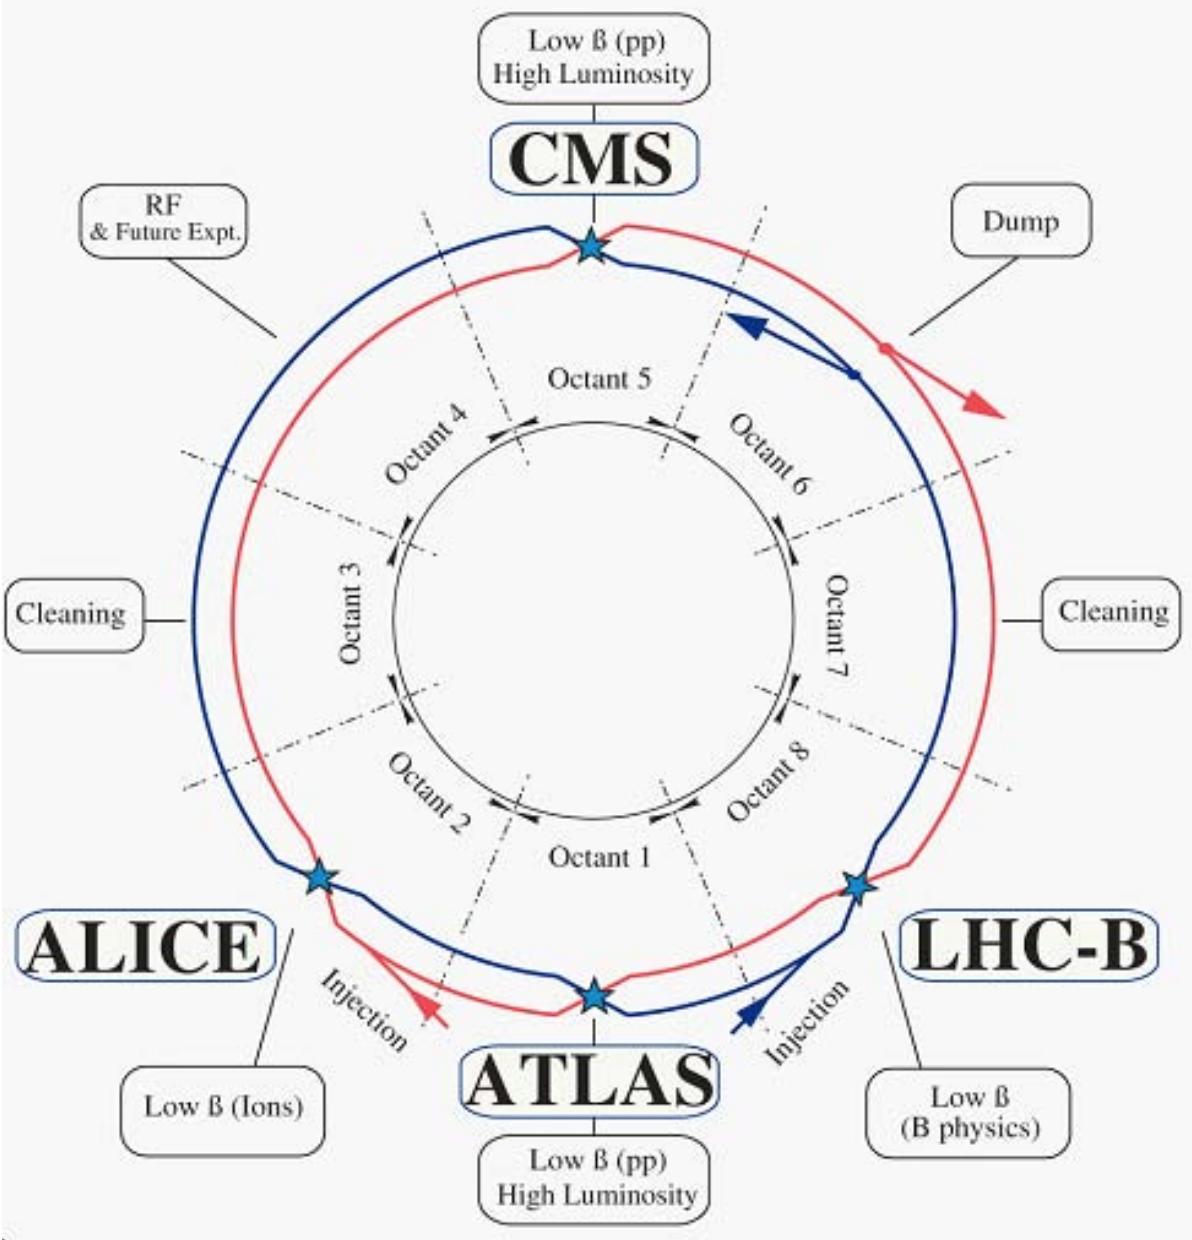
\includegraphics[width=.7\textwidth]{chapters/chapter2_experiment/images/lhc_interaction_points.png}
    \caption[A schematic of the LHC with the various interaction points indicated]{A schematic of the LHC with the various interaction points indicated \cite{lhc}.}
    \label{fig:lhc}
\end{figure}


\section{The ATLAS Detector}

ATLAS \cite{atlas-experiment} is a general-purpose detector designed to reconstruct events from hadrons collided by the \gls{LHC}. With respect to the \gls{IP}, it has forward-backward symmetric cylindrical geometry, and covers a solid angle of almost $4\pi$. It is $\unit{44}{\meter}$ long, $\unit{25}{\meter}$ in diameter, weighs over 7,000 tons, and is located $\unit{100}{\meter}$ underground. 

ATLAS is composed of several nested cylindrical subsystems. Nearest the \gls{IP} is the \glsfirst{ID} (discussed in \ref{ssec:innerdetector}), measuring the trajectory of charged-particles as they bend through a $\unit{2}{T}$ magnetic field created by a solenoid which envelops the \gls{ID} (discussed in \ref{ssec:magnetsystem}). The \gls{ID} is composed of three components: the silicon Pixel Detector, a semiconductor microstrip detector known as the \gls{SCT}, and a straw-tube tracker known as the \gls{TRT}. Outside of the \gls{ID} are the calorimeters (discussed in \ref{ssec:calorimeters}). ATLAS utilizes two calorimeters, a \glsfirst{LAr} calorimeter to measure electromagnetic radiation and a scintillating tile calorimeter to measure hadronic radiation. Beyond the calorimeters is a $\unit{4}{T}$ toroidal magnetic field (also discussed in \ref{ssec:magnetsystem}) and the Muon Spectrometer (discussed in \ref{ssec:muonspectrometer}), which tracks muon trajectories. ATLAS employs a two-stage triggering system, one hardware-based and one software-based, to identify and record interactions containing interesting physics by sending them to the \gls{DAQ} system (discussed in \ref{ssec:tdaq}.)

A schematic of the ATLAS detector can be found in Figure \ref{fig:atlas}.

\begin{figure}[!ht]
    \centering
    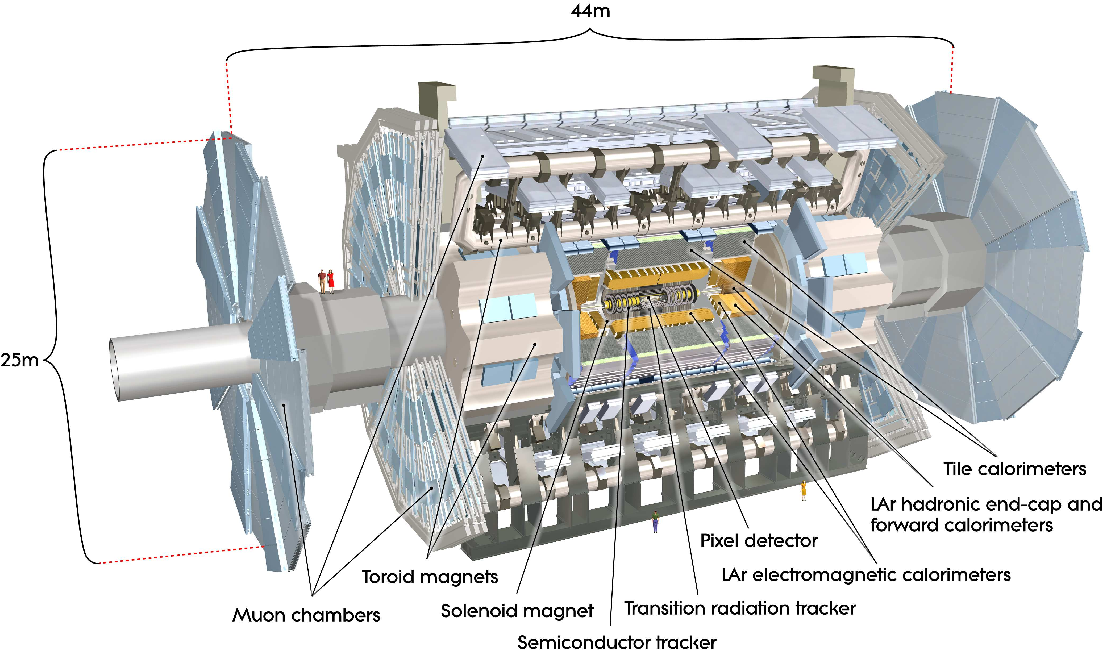
\includegraphics[width=.7\textwidth]{chapters/chapter2_experiment/images/atlas_detector.png}
    \caption[A cut-away schematic the ATLAS detector]{A cut-away schematic the ATLAS detector. Major components and dimensions are labeled \cite{atlas-experiment}.}
    \label{fig:atlas}
\end{figure}

\subsection{The ATLAS Coordinate System}

ATLAS uses a right-handed coordinate system, with the \gls{IP} defining the origin. The $z$-axis is along the beamline, the $x$-axis points toward the center of the \gls{LHC}, and the $y$-axis points upwards, toward Earth's surface.  Transverse quantities such as \pt and \et are calculated in the $x-y$ plane. The half of the detector pointed toward the Saleve is known as the ``A-side'' and has positive $z$ coordinates. The side with negative $z$, pointed toward the Jura, is denoted ``C-side,'' where ``B'' is used to denote the barrel.

Due to the shape of the detector, cylindrical coordinates are also useful for describing position. The azimuthal angle, $\phi$, is measured around the beam axis, with $\phi=0$ lying on the postive $x$-axis. The polar angle, $\theta$, is the angle from the beam axis, where $\theta=0$ is parallel to the beampipe. Commonly, the \textit{pseudorapidity} is used to define position, defined as

\begin{equation}
    \eta = -\ln[\tan(\theta / 2)].
\end{equation}

\begin{figure}[!ht]
    \centering
    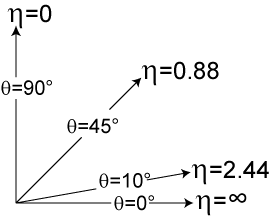
\includegraphics[width=.43\textwidth]{chapters/chapter2_experiment/images/Pseudorapidity2.png}
    \caption[Pseudorapidity distribution shown on a polar grid]{Pseudorapidity distribution shown on a polar grid.}
    \label{fig:pseudorapidity}
\end{figure}

This value is 0 perpendicular to the beamline, and infinite as it approaches the beam axis, as shown in Figure \ref{fig:pseudorapidity}. Occasionally the \textit{rapidity}, defined as
%
\begin{equation}
    y = \frac{1}{2} \log{\frac{E+p_z}{E-p_z}},
\end{equation}
%
is used to describe position as well. Rapidity and pseudorapidity are preferable to the polar angle due to their Lorentz invariance. For massless particles, the rapidity and pseudorapidity are equivalent.

To describe distance between particles, the angle space in pseudorapidity and azimuth is commonly used. It is also Lorentz invariant under longitudinal boosts and defined as
\begin{equation}
    \Dr = \sqrt{\Delta\eta^2 + \Delta \phi^2}.
\end{equation}
%

\subsection{Magnet Systems} \label{ssec:magnetsystem}
In order to measure the charge and momentum of particles in the detector, a magnetic field is used. The curvature of a charged particle as it traverses through a magnetic field can be used to derive the charge to mass ratio. The sign of the charge is determined from the bend of the track.

The magnet system in ATLAS is a hybrid system comprised of four superconducting magnets: a central solenoid, a barrel toroid, and two end-cap toroids. The barrel toroids define the dimensions of the ATLAS detector, extending 26 m along the beam axis, and have an outer diameter of $\unit{22}{\meter}$ \cite{magnet-system-tdr}. A schematic of the components of the magnet system is shown in Figure \ref{fig:magnetSystem}.

% Insert picture
\begin{figure}[!ht]
    \centering
    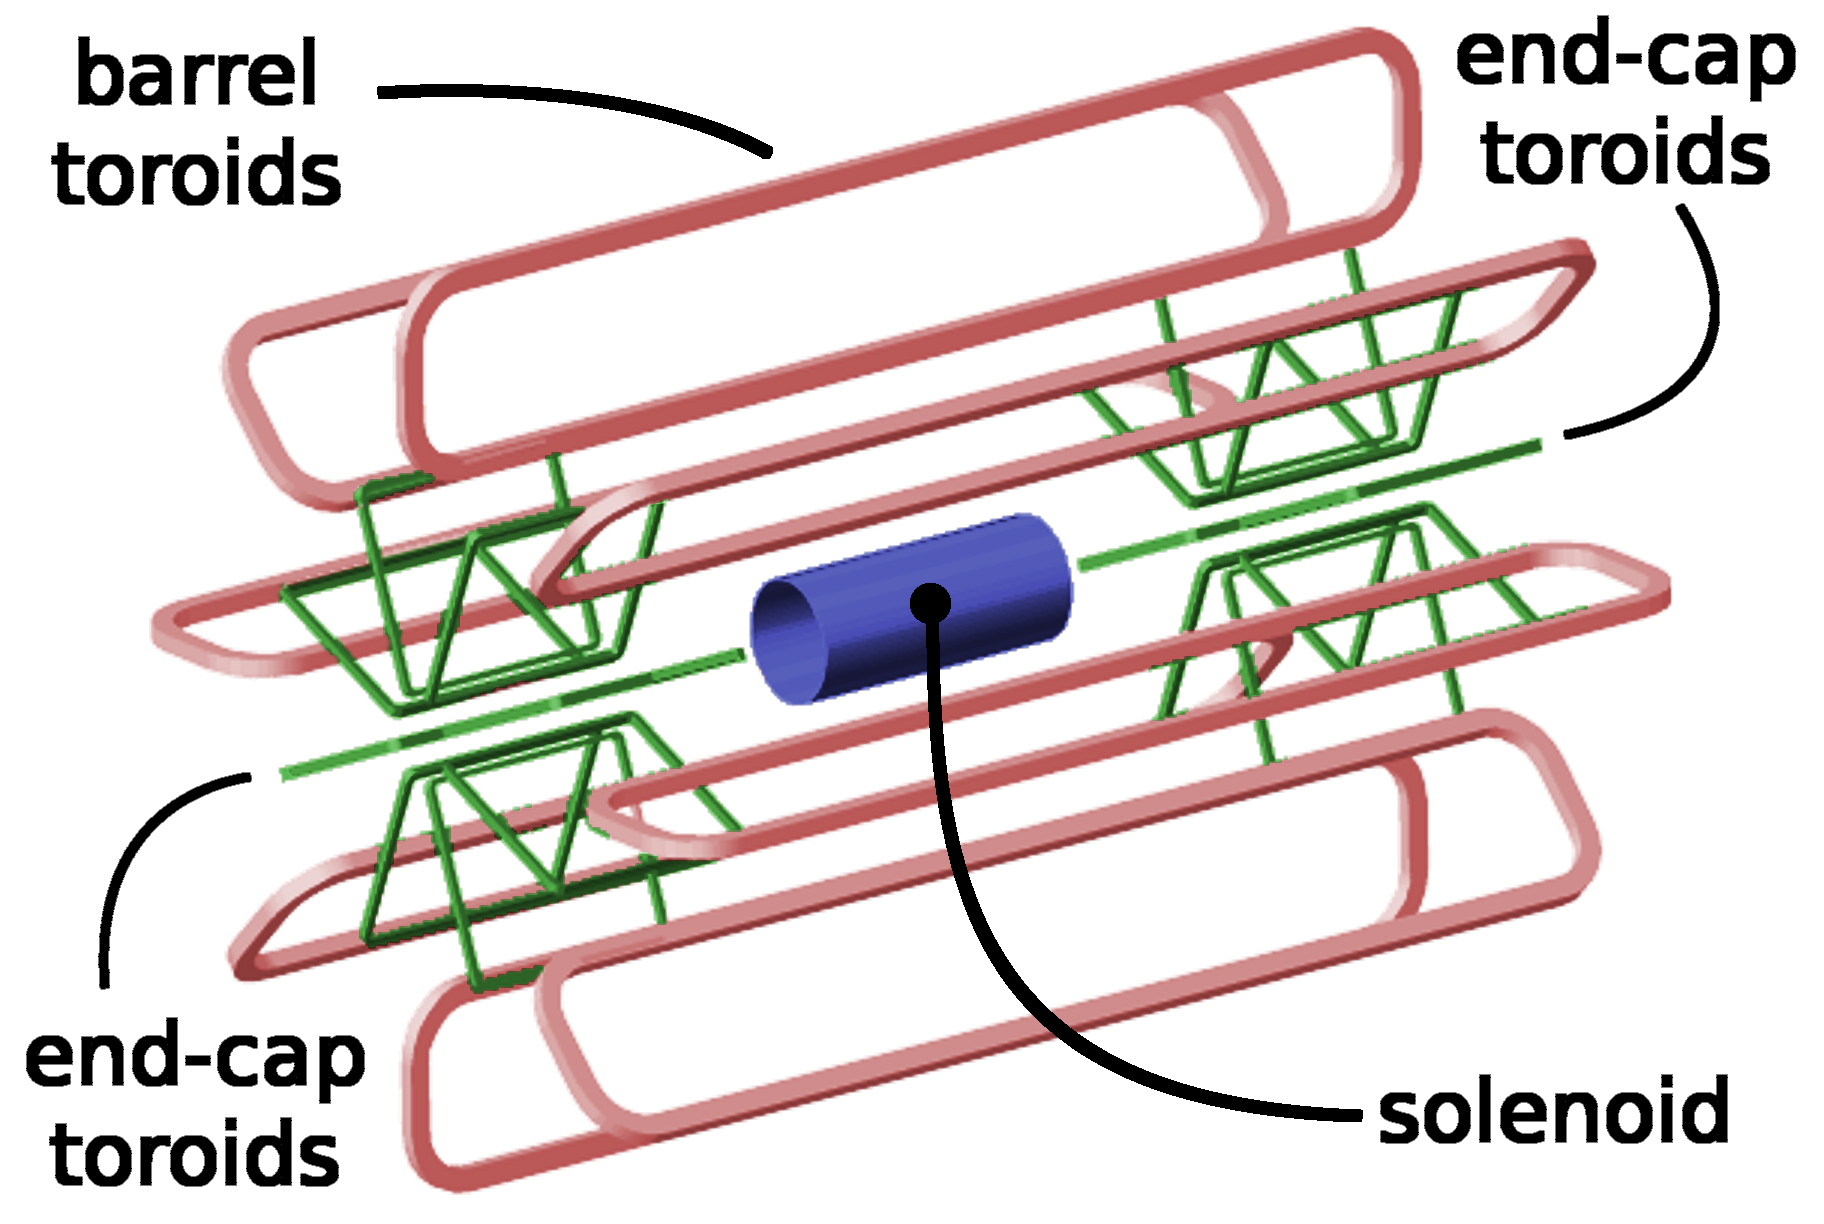
\includegraphics[width=.8\textwidth]{chapters/chapter2_experiment/images/magnetSystems.png}
    \caption[A schematic of the components of the magnet system in the ATLAS detector]{A schematic of the components of the magnet system in the ATLAS detector \cite{magnet-schematic}.}
    \label{fig:magnetSystem}
\end{figure}

\noindent\textbf{Central Solenoid}\\
\indent The central solenoid sits between the \gls{ID} and the \gls{EM} calorimeter and provides a $\unit{2}{\tesla}$ magnetic field. This field is axially symmetric, and causes curvature in charged particles as they move through the \gls{ID}. In order to minimize material before the calorimeters, it was designed to be thin, a single-layer coil wound with 1173 turns with Al-stabilized Nb/Ti conductor. It covers a length of $\unit{5.3}{\meter}$ along the beam axis and has an outer diameter of $\unit{2.63}{\meter}$ \cite{central-solenoid}.

\noindent\textbf{Toroids}\\
\indent The barrel toroid is made up of eight coils of a flat racetrack shape, which provide a symmetric radial magnetic field toward the beam axis, with a peak field of $\unit{3.9}{\tesla}$ \cite{barrel-toroid}. The two end-cap toroids are also composed of eight coils, with a length of 5 m, outer diameter of 10.7 m and an inner bore of 1.65 m, and providing a peak $\unit{4.1}{\tesla}$ field. The end-cap toroids are inserted into the barrel toroid and line up with the center solenoid. The three-toroid design was chosen over a single toroid to maintain easy access to the core of the detector \cite{endcap-toroid}. Together the toroids provide a magnetic field to the muon system, causing curvature in the muon trajectory.


\subsection{Inner Detector}  \label{ssec:innerdetector}

The \gls{ID} \cite{inner-detector-tdr} serves to identify the precise interaction point and trajectory of charged particles. The \gls{ID} is segmented into barrel and end-cap sections along the beam axis. The barrel extends 1.6 m, covering $|\eta| < 1$, and the end-cap sections cover the remainder of the 7 m length. With this setup, the \gls{ID} provides precision tracking up to $|\eta| = 2.5$. It is composed of three subsystems, the Pixel Detector, the \gls{SCT}, and the \gls{TRT}.

\noindent\textbf{Pixel Detector}\\
\indent Nearest the \gls{IP} is the Pixel Detector, which provides high-granularity, high-precision measurements, and is used to determine impact parameters.

Pixel sensors are reversely polarized diodes, created by an n+ implant on an n-doped silicon substrate with dimensions $ \unit{50}{\micron} \times \unit{400}{\micron}$, and a depth of $\unit{250}{\micron}$. The detector has 1,744 modules with 46,080 readout channels per modules, for a total of over 80 million pixels.
    
The innermost layer, the \gls{IBL} \cite{ibl-tdr}, was installed between \RunOne and \RunTwo, during the shutdown that lasted from 2013 to 2015. It takes advantage of smaller modules for finer granularity at $\unit{50}{\micron} \times \unit{250}{\micron}$. Additionally, it is located closer to the interaction point, at a distance of $R=\unit{33.25}{\mm}$, compared to the previous first layer at $R=\unit{50.5}{\mm}$. The smaller distance between the beamline and first detector layer helps for finding displaced vertices from b-jets and photons converting into an $e^+e^-$ pair.

\noindent\textbf{SemiConductor Tracker}\\
\indent The \gls{SCT} provides measurements at intermediate range from the \gls{IP}, vital for momentum, impact parameter, and vertex position measurements. It is composed of a barrel region and two end-caps, covering the distance $R=\unit{300}{\mm}$ to $R= \unit{520}{\mm}$ from the \gls{IP}. \gls{SCT} modules are made up of four strip sensors, two on each side, oriented at an angle of $\unit{40}{\mrad}$ from each other. The sensors are single-sided p-in-n microstrip detectors on silicon wafers. The barrel is constructed of 2112 modules in four layers that are equally spaced, and each end-cap is constructed of 988 modules over nine disks. Collectively, the \gls{SCT} has about 6 million silicon strips.

\noindent\textbf{Transition Radiation Tracker}\\
\indent The \gls{TRT} is the outermost subdetector of the \gls{ID}, spanning from a distance $R=\unit{554}{\mm}$ to $R= \unit{1082}{\mm}$ from the \gls{IP}, and pseudorapidity range $|\eta| < 2.0$. The \gls{TRT} contributes to the momentum measurement, aids in pattern recognition for tracking, and provides discrimination between electrons and hadrons. It is a proportional drift tube composed of 372,032 straws, each with a $\unit{4}{\mm}$ inner diameter. In the barrel, the straws have a length of $\unit{144}{\cm}$ and are arranged parallel to the beam axis. In the end-cap, straws are $\unit{37}{\cm}$ long, and arranged into 18 wheels, radially from the beam axis.

The straws are filled with a gaseous mixture\footnote{This was the design gas mixture, as described in the \gls{ID} Technical Design Report, Reference \cite{inner-detector-tdr}. During \RunTwo, straws with leaks were filled with 70\% Ar gas, rather than Xe due to cost. Ar provides similar tracking performance as Xe, but a worse efficiency absorbing transition radiation X-rays.} composed of 70\% Xe, 27\% CO\textsubscript{2}, and 3\% O\textsubscript{2}. As a charged particle penetrates the straw, it deposits energy into the gas and creates electron-ion pairs. The electrons drift to the center wire, while the ions drift to the inner wall of the straw. The drifting charge produces an electrical signal, which is then compared to a low and high threshold. The low threshold is used to measure drift time, which is used to derive position of incidence. The high threshold is used to identify large energy deposits from transition radiation X-rays, which is useful to discriminate charged pions from electrons.

For momentum measurement, the \gls{TRT} provides measurements equivalent to a single point with precision of $\unit{50}{\micron}$. For tracking, it provides around 36 hits per track. For electron-hadron discrimination, it has a pion rejection factor of between 15 and 200 (depending on $\eta$) for pions with $\pt > \unit{20}{\GeV}$, at an electron efficiency of 90\%.


\begin{figure}[!thp]
    \begin{minipage}[c]{.53\textwidth}
        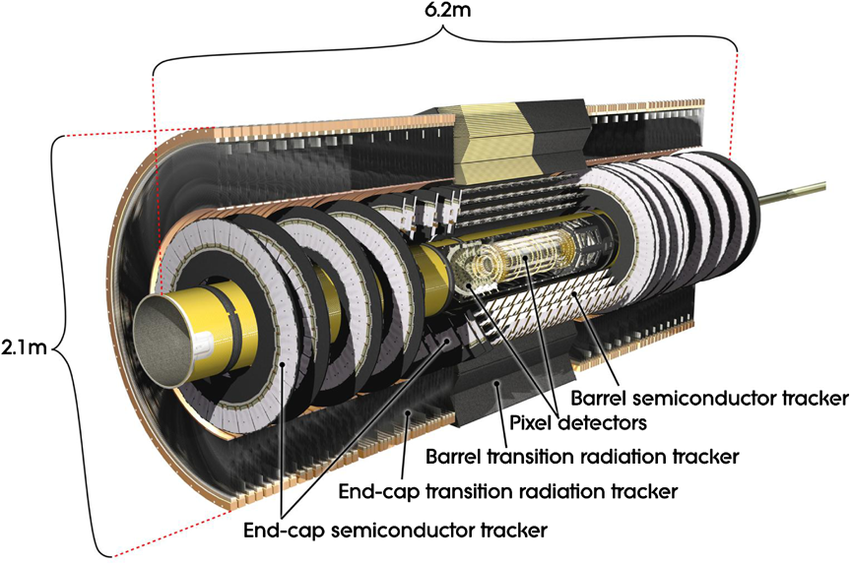
\includegraphics[width=\textwidth]{chapters/chapter2_experiment/images/id_slice.png}
    \end{minipage}
    \begin{minipage}[c]{.45\textwidth}
        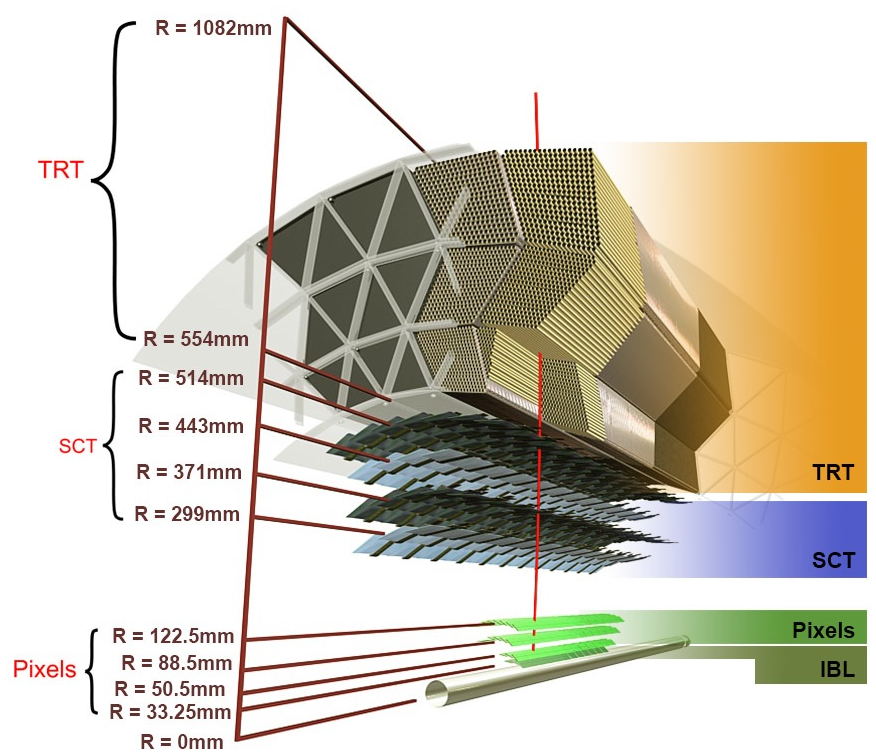
\includegraphics[width=\textwidth]{chapters/chapter2_experiment/images/id_layer.png} 
    \end{minipage}
    \caption[Schematic of the components of the ATLAS \gls{ID}]{Schematic of the components of the ATLAS \gls{ID}. A scale cutaway view of the \gls{ID} with the Pixel and \gls{SCT} (left) \cite{pixel-electronics}, and a layer-by-layer view of the \gls{ID} subdetectors (right) \cite{id-perf2015}.}
\end{figure}
    

\subsection{Calorimeters} \label{ssec:calorimeters}
The calorimeter system in ATLAS serves to measure the energy of particles absorbed by their active material. ATLAS employs calorimeters targeting different types of particle showering: the \gls{LAr} \gls{EM} calorimeter targets \gls{EM} showers from photons and electrons, while the hadronic Tile calorimeter targets hadronic showers. The \gls{EM} calorimeter lies outside the \gls{ID} and central solenoid, and the hadronic calorimeter is outside of the \gls{EM} calorimeter.  A schematic of the calorimeter can be found in Figure \ref{fig:calorimeter}.


\begin{figure}[!ht]
    \centering
    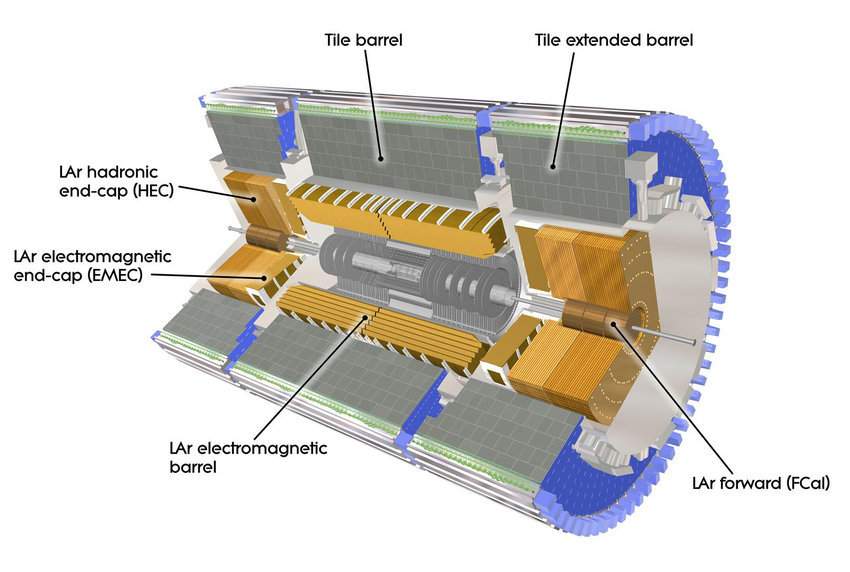
\includegraphics[width=.7\textwidth]{chapters/chapter2_experiment/images/calorimeter.jpeg}
    \caption[A schematic of the calorimeters in the ATLAS detector]{A schematic of the calorimeters in the ATLAS detector \cite{atlas-experiment}.}
    \label{fig:calorimeter}
\end{figure}

\begin{figure}[!ht]
    \centering
    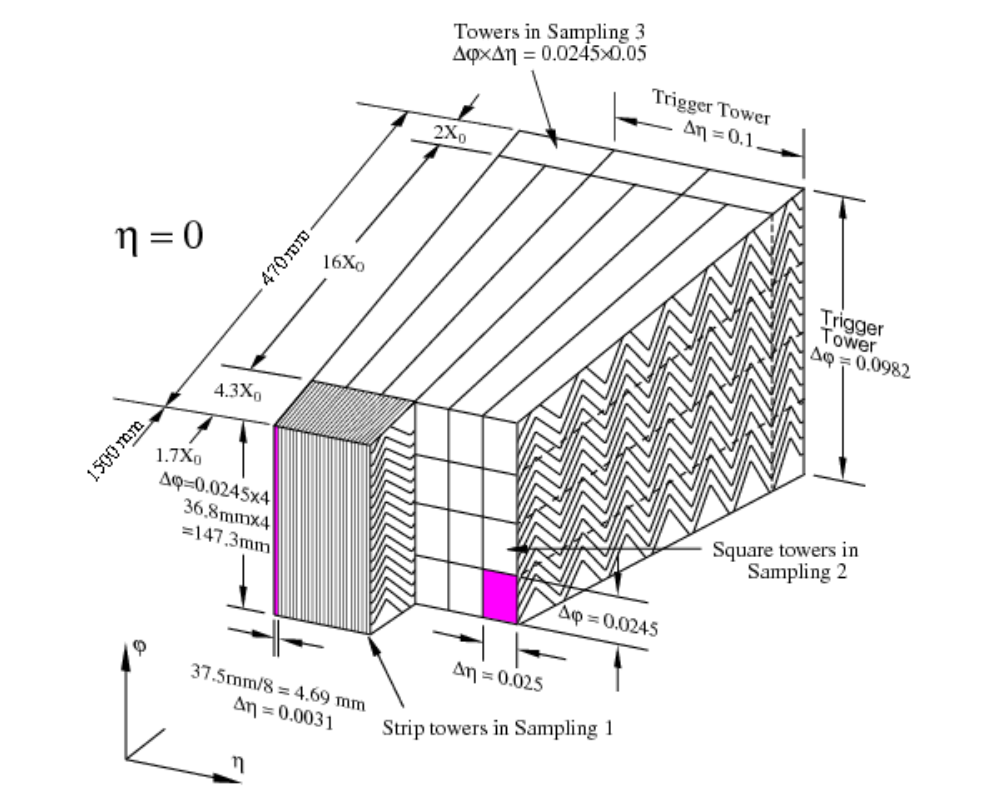
\includegraphics[width=.9\textwidth]{chapters/chapter2_experiment/images/lar.png}
    \caption[A sketch of the \gls{LAr} \gls{EM} calorimeter]{A sketch of the \gls{LAr} \gls{EM} calorimeter \cite{lar-tdr}.}
    \label{fig:lar}
\end{figure}

\noindent\textbf{Electromagnetic Calorimeter}\\
\indent The electromagnetic calorimeter is a \gls{LAr} sampling calorimeter. Upon interacting with the \gls{LAr} active material, photons will interact dominantly by creation of $e^+e^-$ pairs above 5 MeV. Below that threshold, photons interact via the photoelectric or Compton effect. For electrons, interaction occurs via bremsstrahlung at energies above 1 MeV, causing the electron to radiate photons and decelerate. This continues for subsequent daughter particles and has a showering effect in the calorimeter \cite{detectors-for-radiation}.

The \gls{LAr} \gls{EM} calorimeter features absorbers with an ``accordion'' style geometry, and read-out electrodes. The accordion geometry provides gap-less azimuthal ($\phi$) symmetry. The \gls{EM} calorimeter is composed of three regions, the \gls{EMB} and two \glspl{EMEC}, each with their own cryostat.

The \gls{EMB} uses lead-stainless steel converters as the passive material and covers $|\eta| < 1.5$. It is split into two half-barrels, meeting at $|\eta| = 0$, each with 1024 converters and electrodes. Longitudinally, the \gls{EMB} is divided into three layers. The first strip layer is very finely segmented in $\eta$ to provide precision position information, with granularity $0.003 \times 0.1$ in $\Delta\eta \times \Delta \phi$. The second layer has a wider segmentation, $0.025 \times 0.025$, and absorbs the bulk of the \gls{EM} shower. The last layer has even lower granularity in $\eta$, $0.05 \times 0.025$, and serves to pick up the \gls{EM} shower tails. In total, these three layers cover more than $22$ \gls{X_0} and have 101,760 total channels.

The \gls{EMEC} also uses lead-stainless steel as the passive material and is comprised of two concentric wheels, an inner wheel covering $1.4 < |\eta| < 2.5$, and an outer wheel covering $2.5 < |\eta| < 3.2$, and covers $>24$ \gls{X_0}. Between the \gls{EMB} and \gls{EMEC}, a transition crack spans $1.37 < |\eta| < 1.52$, which is also used to service the detector.

In front of the calorimeter cryostats, a presampler is used to correct for energy lost before particles reach the calorimeters. The presampler uses thin copper electrodes and \gls{LAr} as the active material, with a layer of 1 cm thickness in the barrel and 5 mm in the end-caps, and granularity of $0.025 \times 0.1$ in $\Delta\eta \times \Delta \phi$ \cite{lar-tdr}.


A sketch of the composition of the \gls{EM} calorimeter can be found in Figure \ref{fig:lar}.

\begin{figure}[!ht]
    \centering
    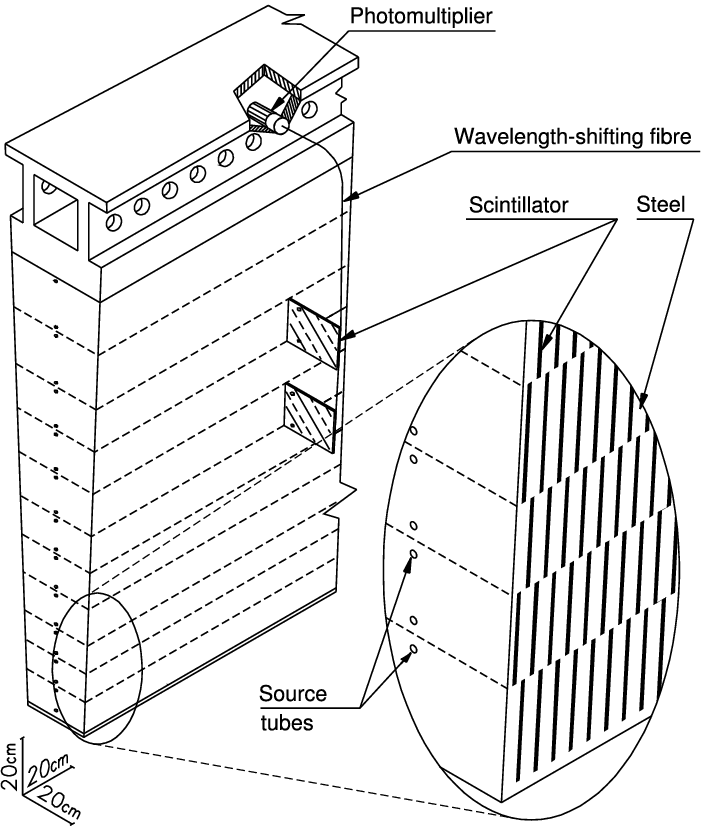
\includegraphics[width=.65\textwidth]{chapters/chapter2_experiment/images/tile.png}
    \caption[A sketch of the hadronic Tile calorimeter]{A sketch of the hadronic Tile calorimeter \cite{tile-tdr}.}
    \label{fig:tile}
\end{figure}


\noindent\textbf{Hadronic Calorimeter}\\
\indent As hadrons interact with matter, their scattering produces secondary hadrons as well as protons and neutrons. These also decay and this cascade, known as a hadronic shower, will continue until the energy of the decay products is small enough to be halted by ionization energy loss or absorbed in a nuclear process.

\indent The hadronic Tile Calorimeter is designed to measure the energy of particles by using these decays, employing steel as the absorber and scintillating tiles as the active material. The scintillators transmit light via fiber optics to \glspl{PMT}. The hadronic calorimeter is composed of three regions, the central barrel, covering $|\eta| < 1.0$, and two extended barrels on either side of the central barrel, covering $|\eta| > 1.0$. Each of these three regions have 64 azimuthal modules, and 3 layers longitudinally. The first two layers have granularity $0.1 \times 0.1$ in $\Delta\eta \times \Delta \phi$, while the third is $0.2 \times 0.1$. The thickness covers more than 9.7 \gls{intLen}. A sketch of the composition of the Tile Calorimeter can be seen in Figure \ref{fig:tile}.

A \gls{HEC} also works to detect hadronic decays, covering pseudorapidity range of $1.4 < |\eta| < 3.2$. There are two wheels per end-cap, located behind the \glspl{EMEC} and sharing their cryostats. The \gls{HEC} uses \gls{LAr} as the active material, and copper plates as the passive material. Each end-cap features 32 wedge shaped modules, and two segments in depth, making four total samplings per end-cap \cite{lar-tdr}.


\noindent\textbf{\gls{FCal}}\\
\indent In order to get precise measurements of \gls{MET}\footnote{\gls{MET} is not used in the present work, however is used in many ATLAS analyses. It aims to measure those particles which do not interact with the detector, such as neutrinos or many \gls{BSM} signatures. Since the two colliding partons (defined in Section \ref{ssec:eventgen}) cancel out each other's momentum, the initial transverse momentum is 0. Because of the law of conservation of momentum, the sum of momentum of the final state particles must also sum to 0. If the reconstructed particles do not, then the remainder is defined as \gls{MET}.}, full $\eta$ coverage is necessary. The \gls{FCal} covers the most forward regions, covering $3.1 < |\eta| < 4.9$. It is three modules deep, covering 10 \gls{intLen}, the first module made of copper, targeting \gls{EM} depositions, and the outer two made of tungsten targeting hadronic depositions.


\subsection{Muon Spectrometer} \label{ssec:muonspectrometer}
The \glsfirst{MS} \cite{muon-tdr} is the outermost layer of the ATLAS detector, aiming to track muons via independent triggering (up to $|\eta| < 2.4$) and momentum measurement (up to $|\eta| < 2.7$). Triggers based on the \gls{MS} are combined with information from the \gls{ID} to make the final trigger decision, so good timing resolution is imperative.

Timing information in the \gls{MS} is collected in the \glspl{RPC} and \glspl{TGC}. These both feature timing resolution better than 4.5 ns. The \glspl{RPC} cover the barrel ($|\eta| < 1.05$) region while the \glspl{TGC} covers the end-cap ($1.0<|\eta|<2.4$).


Momentum information is provided through Al tubes 30 mm in diameter and filled with a 0.05 mm gold-plated tungsten wire in the center, called a \glsfirst{MDT}. Three layers of \glspl{MDT} cover the central region of the \gls{MS}, at $|\eta| < 2.7$. In the forward region, $2.0<|\eta|<2.7$, the first \glspl{MDT} layer is replaced by multi-wire proportional chambers with precision cathode strips, known as \glspl{CSC}.

\begin{figure}[!ht]
    \centering
    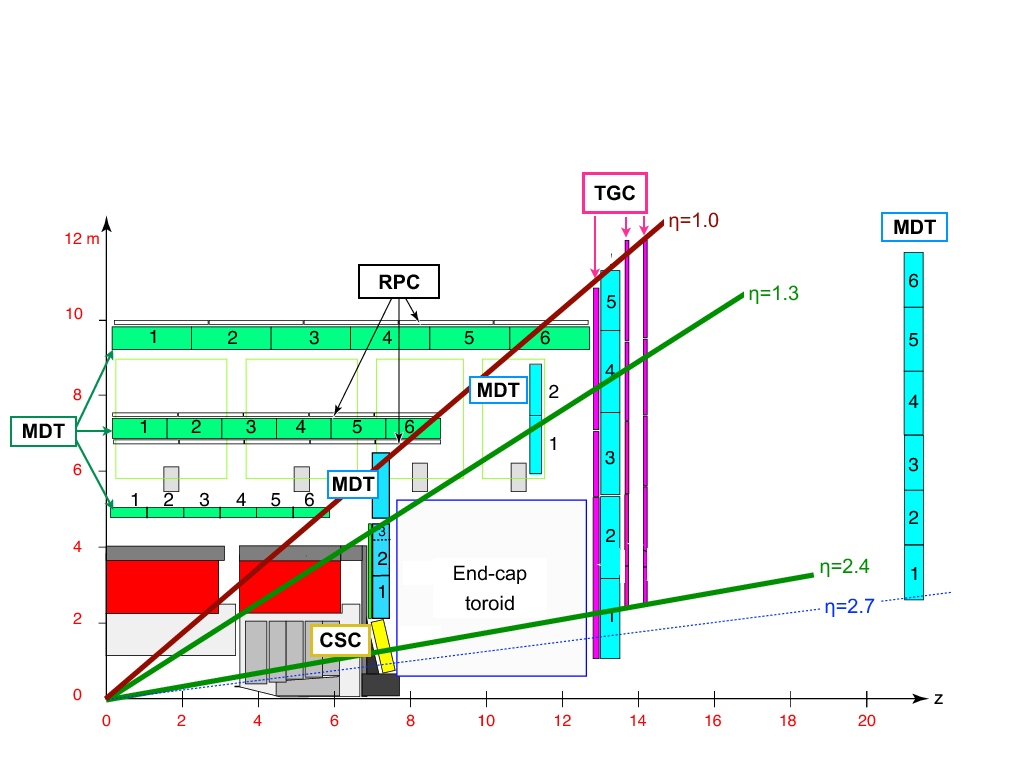
\includegraphics[width=.9\textwidth]{chapters/chapter2_experiment/images/muon_detector.png}
    \caption[A schematic of a quarter of the \gls{MS}]{A schematic of a quarter of the \gls{MS}. The described systems, the \gls{RPC}, \gls{TGC}, \gls{MDT}, and \gls{CSC} are labeled \cite{muon-performance2015}.}
    \label{fig:muon-schematic}
\end{figure}

A schematic of the \gls{MS} is found in Figure \ref{fig:muon-schematic}.

\subsection{Trigger and Data-Acquisition} \label{ssec:tdaq}

Dataflow and storage are a major challenge for ATLAS. Bunches of protons interact every 25 ns, a rate of 40 MHz. On average, raw event contains about 1.6 MB \cite{ATLASfact-sheet}; recording all of those interactions would not be possible, nor desirable since they are dominated by soft collisions processes which do not yield interesting physics. To isolate events which are desirable to record, ATLAS utilizes a two-stage trigger system \cite{triggerTDR}.

First, the \gls{L1} trigger receives events at 40 MHz and makes quick decisions based on coarse information. This trigger system is hardware based, constructed out of custom electronics, and targets specific features in the calorimeter or muon system. From hits in each detector, candidate physics objects (electrons, photons, muons, jets, and \gls{MET}) are formed, and events are accepted or rejected based on features of these candidates in order to get to an average event rate of between 75 and 100 kHz, a reduction factor of about 400. Additionally in this process, \glspl{ROI}, cones in $\eta \times \phi$ containing interesting physics, are identified, and passed down the trigger chain.

The second stage of the trigger is software-based, known the \gls{HLT}. On average, the \gls{HLT} has $\unit{200}{\micro\second}$ per event to make decisions. It uses the \gls{ROI} provided from \gls{L1} to make decisions based on fast algorithms by reconstructing partial events within that region, reconstructing just 2\%-6\% of the total event data. At this stage, the event rate is reduced to around $\unit{3}{\kHz}$.

Events that pass this stage then are reconstructed with offline-like algorithms, allowing for triggering on sophisticated signatures (e.g. \gls{MET}) and the final trigger decision is made using those objects. This produces a final output between 500 and 1000 Hz. Events selected by the \gls{HLT} are saved to the offline system based on their trigger decision, known as data streams. A schematic of the pipeline for trigger decisions in conjunction with the \gls{DAQ} system is shown in Figure \ref{fig:trigger-schematic}.


\begin{figure}[!ht]
    \centering
    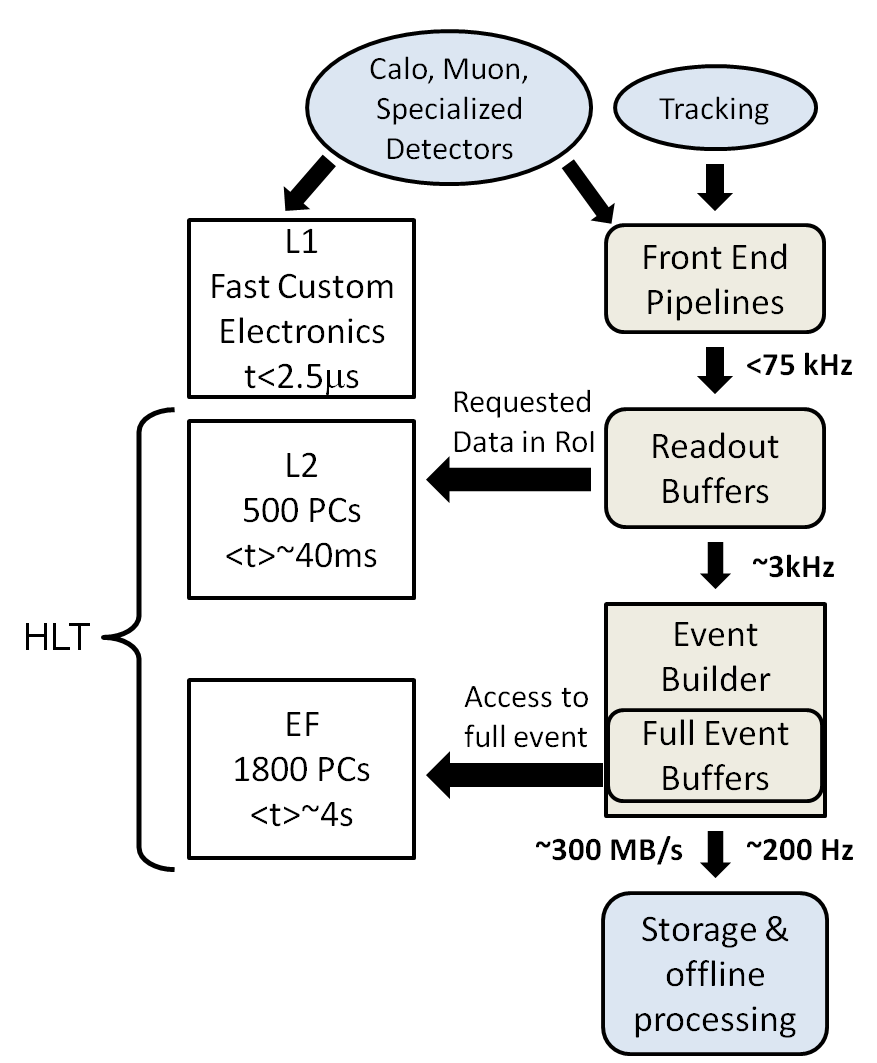
\includegraphics[width=.80\textwidth]{chapters/chapter2_experiment/images/trigger.png}
    \caption[The ATLAS Trigger and DAQ system during the \RunTwo data taking period]{The ATLAS Trigger and DAQ systems during the \RunTwo data taking period. Inputs from the various subsystems start at the top right, where they are then passed to the \gls{L1} trigger, shown in the upper left. Events passing that are sent to the \gls{HLT} (lower left), while simultaneously data are passed from the \glspl{ROD} to the \gls{ROS} on \gls{L1} accepts. They are buffered and available for the \gls{HLT} to sample. These accepted events are then sent to storage via the Data Logger. Event and data rates are shown for each step on the left and right, respectively \cite{trigger-run2}.}
    \label{fig:trigger-schematic}
\end{figure}

% TODO: FTK?